\makeheading{量子纠缠的第一张图像}


\begin{multicols}{2}

有时,两个相互作用的粒子——比如两个通过分束器的光子,无论被分隔到多么遥远,它们都可以保持联系,并瞬间共享它们的物理状态.这种神秘的联系被称为\qiangdiao{量子纠缠},它支撑了整个量子力学领域.爱因斯坦曾将这一现象称为\qiangdiao{“鬼魅般的超距作用”}.

Sometimes two interacting particles, such as two photons passing through a beam splitter, can stay connected, no matter how far apart, and share their physical states instantaneously.This mysterious connection, called \qiangdiao{quantum entanglement}, underpins the whole field of quantum mechanics.Einstein once called this phenomenon \qiangdiao{"ghostly action at a distance."}

\begin{figure}[H]
    \centering
    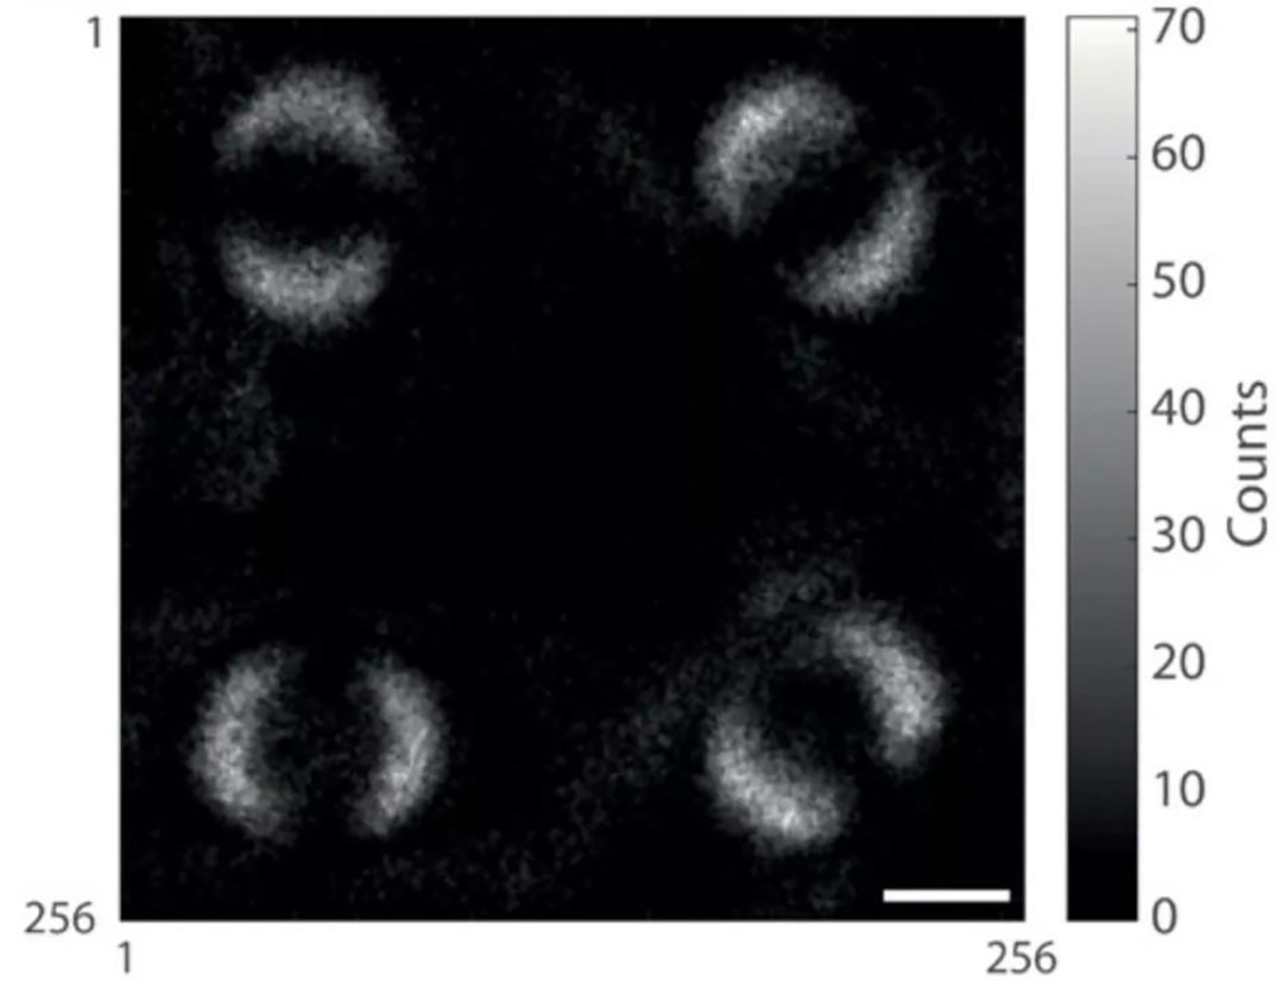
\includegraphics[width=0.7\linewidth]{IMG/201907/01.jpg}
    \caption{}
    
\end{figure}

爱因斯坦之所以称之为“鬼魅”,是因为两个相距甚远的纠缠粒子间的相互作用表现出的瞬时性,似乎与他的狭义相对论并不兼容.后来,约翰·贝尔(John Bell)正式提出了这种\qiangdiao{非局域}相互作用的概念,描述了一种能展现这种鬼魅效应的强纠缠形式——被称为\qiangdiao{贝尔纠缠}.一直以来,虽然贝尔纠缠在量子计算和密码学等许多实际应用中都得到了应用,但我们从来没有捕获它的图像.于7月12日发表在《科学进展》上的论文中,格拉斯哥大学的一组物理学家描述了他们如何让这种“鬼魅现象”首次出现在图像中,这是第一次捕捉到量子纠缠的视觉证据.

Einstein called it "ghostly" because the instantaneous nature of the interaction between two distant entangled particles did not seem compatible with his theory of special relativity.Later, John Bell formally proposed the concept of this \qiangdiao{nonlocal} interaction, describing a form of strong entanglement --known as \qiangdiao{Bell entanglement} -- that can display this ghostly effect.Although bell entanglement has been used in many practical applications, such as quantum computing and cryptography, we have never captured an image of it.In a paper published in the July 12 issue of \textit{Science Advances}\/, a team of physicists from the university of Glasgow describe how they made the "ghostly phenomenon" appear in images for the first time, capturing visual evidence of quantum entanglement.

他们设计了一个系统(\textit{实验系统的设置如图2所示}),一个波长为355 纳米的准连续激光通过了一个BBO 晶体(\textit{偏硼酸钡晶体}),从而通过自发参量下转换(SPDC)过程产生了在空间上纠缠的光子对.这两个波长为 710 纳米的光子在一个分束器(BS)上分离,并沿着光学系统中的两条不同的光路传播.

They designed a system (\textit{as shown in Fig.2}\/) quasi-continuous in laser which with a a wavelength of 355 nanometers passes through a BBO crystal (\textit{barium metaborate crystal}\/), generating spatially entangled pairs of photons through a spontaneous parametric downconversion (SPDC) process.The two 710-nanometer photons are separated on a beam splitter (BS) and travel along two different paths in the optical system. 

第一个光子被放置于晶体的成像面上的空间光调制器(SLM)反射,并在被一个单模光纤收集之前,显示出一个相位物体,然后在被光纤收集之后,再被一个单光子雪崩二极管(SPAD)探测到.另一个光子沿着另一条光路传播,它被一个放置在晶体的傅里叶平面(\textit{相当于物体的傅里叶平面})的SLM反射.然后,这个光子会通过一个长约20米的延迟线(\textit{Delay line}\/)传播,最终被一个增强型电荷耦合检测器(ICCD)相机检测到.

The first photon is reflected by a spatial light modulator (SLM) placed on the imaging surface of the crystal, showing a phase object before being collected by a single-mode fiber, and then detected by a single-photon avalanche diode (SPAD) after being collected by the fiber.Another photon travels along another path, and it is reflected by a SLM placed in the Fourier plane of the crystal (\textit{the Fourier plane of the object}\/).The photon then travels through a Delay line about 20 meters long and is detected by an enhanced charge coupled detector (ICCD) camera. 

\end{multicols}

\begin{figure}[t]
    \centering
    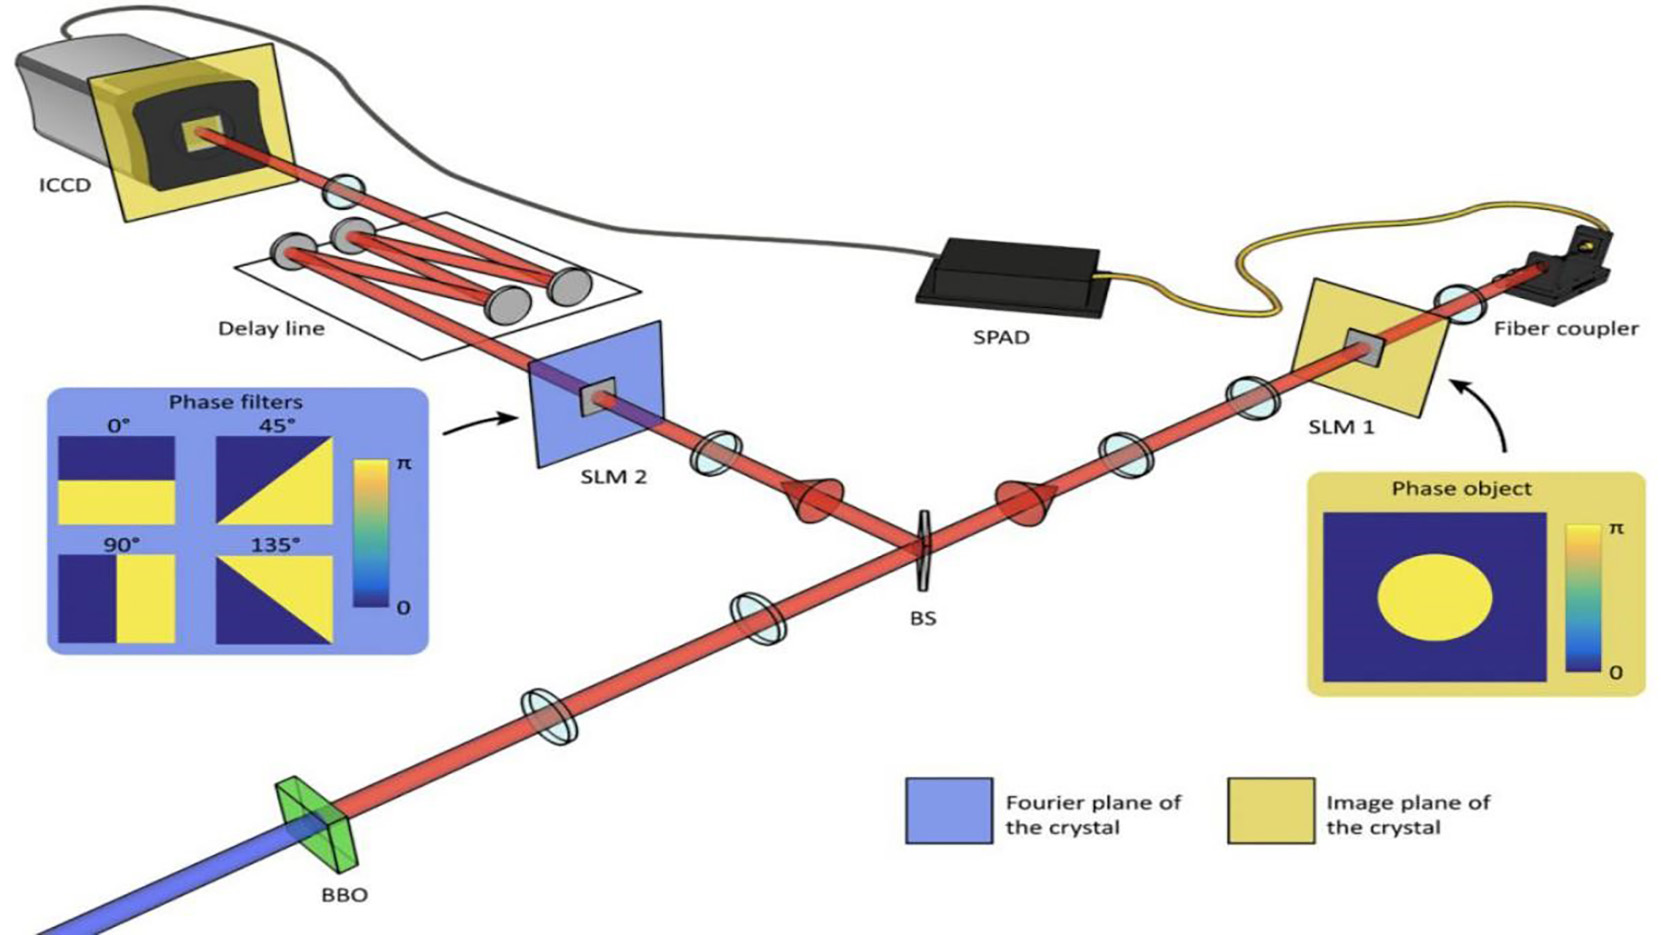
\includegraphics[width=0.9\linewidth,height=9.5cm]{IMG/201907/02.jpg}
    \caption{\textit{实验人员设置了一个超灵敏的照相机,能够检测到单个光子,只有当同时捕捉到一个光子和与它纠缠的另一个粒子时,照相机才会拍下照片,从而记录下了一个可见的光子纠缠记录.}}
    
\end{figure}

\begin{multicols}{2}

相机会根据放置在第一条光路上的 SPAD 探测到光子的情况而被有条件地触发的.而延迟线则确保了从ICCD相机所捕获的图像与 SPAD检测到的图像是同步的.第二条光路中延迟线的存在弥补了相机的触发延迟,并确保了第二个光子入射到相机上的时间的精确度,从而记录下了一个可见的光子纠缠记录.物理学家保罗-安托万·莫罗(Paul-Antoine Moreau) 是这篇论文的第一作者,他说:“我们成功捕捉到的这张照片,优雅地展示了自然的一个基本属性,这是这个属性第一次以图像的形式出现……这是一个令人兴奋的结果,它将可以用于革新量子计算的新兴领域,带来新型的成像方法.” 

The ICCD phase is triggered conditionally by the detection of photons by the SPAD placed on the first light path.The delay line ensures that the images captured from the ICCD camera are synchronized with those detected by the SPAD.The existence of a delay line in the second light path compensates for the trigger delay of the camera and ensures the accuracy of the time of the second photon incident to the camera, thus recording a visible photon entanglement record.Physicist paul-antoine Moreau, the paper's lead author, said: 'this is the first time that an essential property of nature has been captured in an image...This is an exciting result that could be used to revolutionize the emerging field of quantum computing and lead to new imaging methods."

\end{multicols}

\noindent \qiangdiao{参考链接}

\noindent\url{[1]https://phys.org/news/2019-07-scientists-unveil-first-ever-image-quan tum.html }

\noindent\url{[2]https://advances.sciencemag.org/content/5/7/eaaw2563}\vfill

\ADxinhangdao

\newpage
\makeheading{为什么彩条牙膏的颜色不会混合}
\begin{multicols}{2}

每天刷牙的时候,你有没有想过彩条牙膏的彩条是怎么来的?为什么不同颜色的彩条在牙膏管子里不会混在一起?
其实,如今的彩条牙膏在管子里的样子和挤出来的样子差不多.你可以切开一个看看.如果把彩条牙膏冻住,然后剪开包装,就是这样的:
\begin{figure}[H]
    \centering
    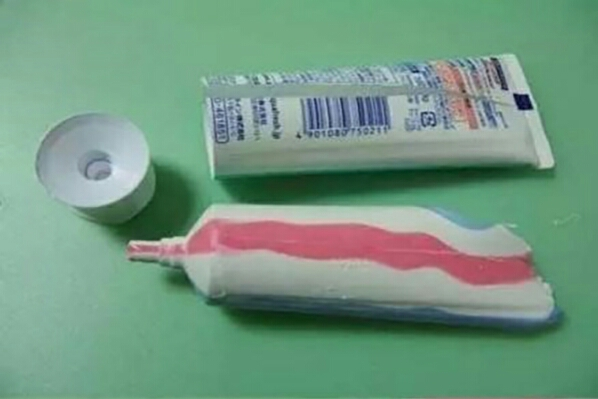
\includegraphics[width=0.333\linewidth]{IMG/201907/03a.jpg}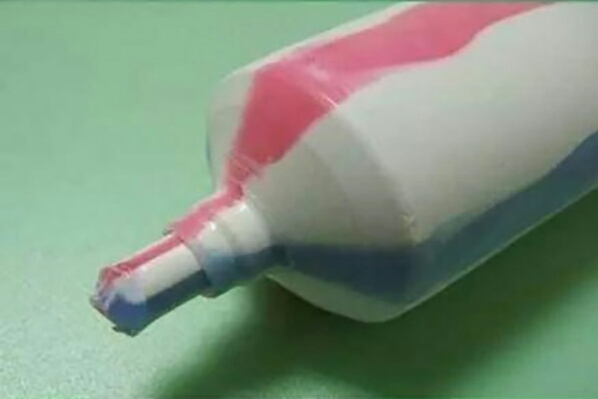
\includegraphics[width=0.333\linewidth]{IMG/201907/03b.jpg}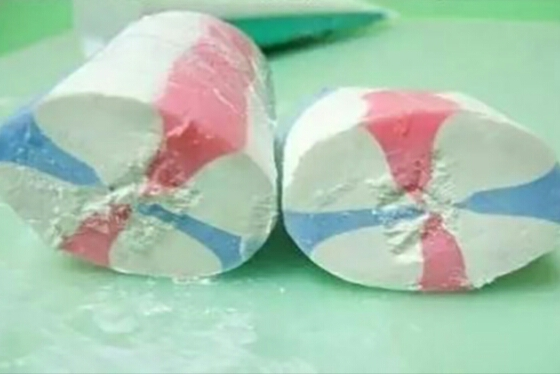
\includegraphics[width=0.333\linewidth]{IMG/201907/03c.jpg}
    \caption{}
    
\end{figure}


\section*{彩条牙膏是怎么制作的?}

在工厂里的时候,机器把不同颜色的彩条分别装到一个中间有隔板的管子里,不同颜色的彩条被隔板隔开.接着就像做冰淇淋那样,机器把所有彩条一起打到牙膏管子里.


那么问题就来了,不同颜色的彩条在牙膏里怎么不会混合在一起,尤其是在被挤了很多次以后?这要分成静止状态和挤牙膏2个情况讨论.静止的牙膏里的彩条不变色,主要是因为2个因素——牙膏的流体物理性质以及彩条所用的色素.牙膏是一种\qiangdiao{宾汉流体}(\textit{Bingham Plastic}\/),属于非牛顿流体.除了牙膏,血液、酸奶、蛋黄酱都是宾汉流体.宾汉流体的一个超强属性就是,在不受力,比如没有被挤压的情况下,它可以像固体一样基本不流动.而受到了一定程度的挤压后,宾汉流体才能开始流动.因此当牙膏没有被你挤的时候,彩条能保持比较稠密的状态,比较接近不能流动的固体,可以在牙膏管里互不干扰.另外,在一般情况下,不同颜色的染料会发生\qiangdiao{渗色}(\textit{bleeding}\/)的现象.彩条牙膏的生产厂家为了防止彩条互相渗色,常用聚乙烯包裹染料,使它们变得稳定.这就是静止的牙膏彩条不会混合的两大原因.
\end{multicols}

\begin{table}[h]
    \centering
    \caption{\textit{红色和蓝色是常用的彩条颜色}}
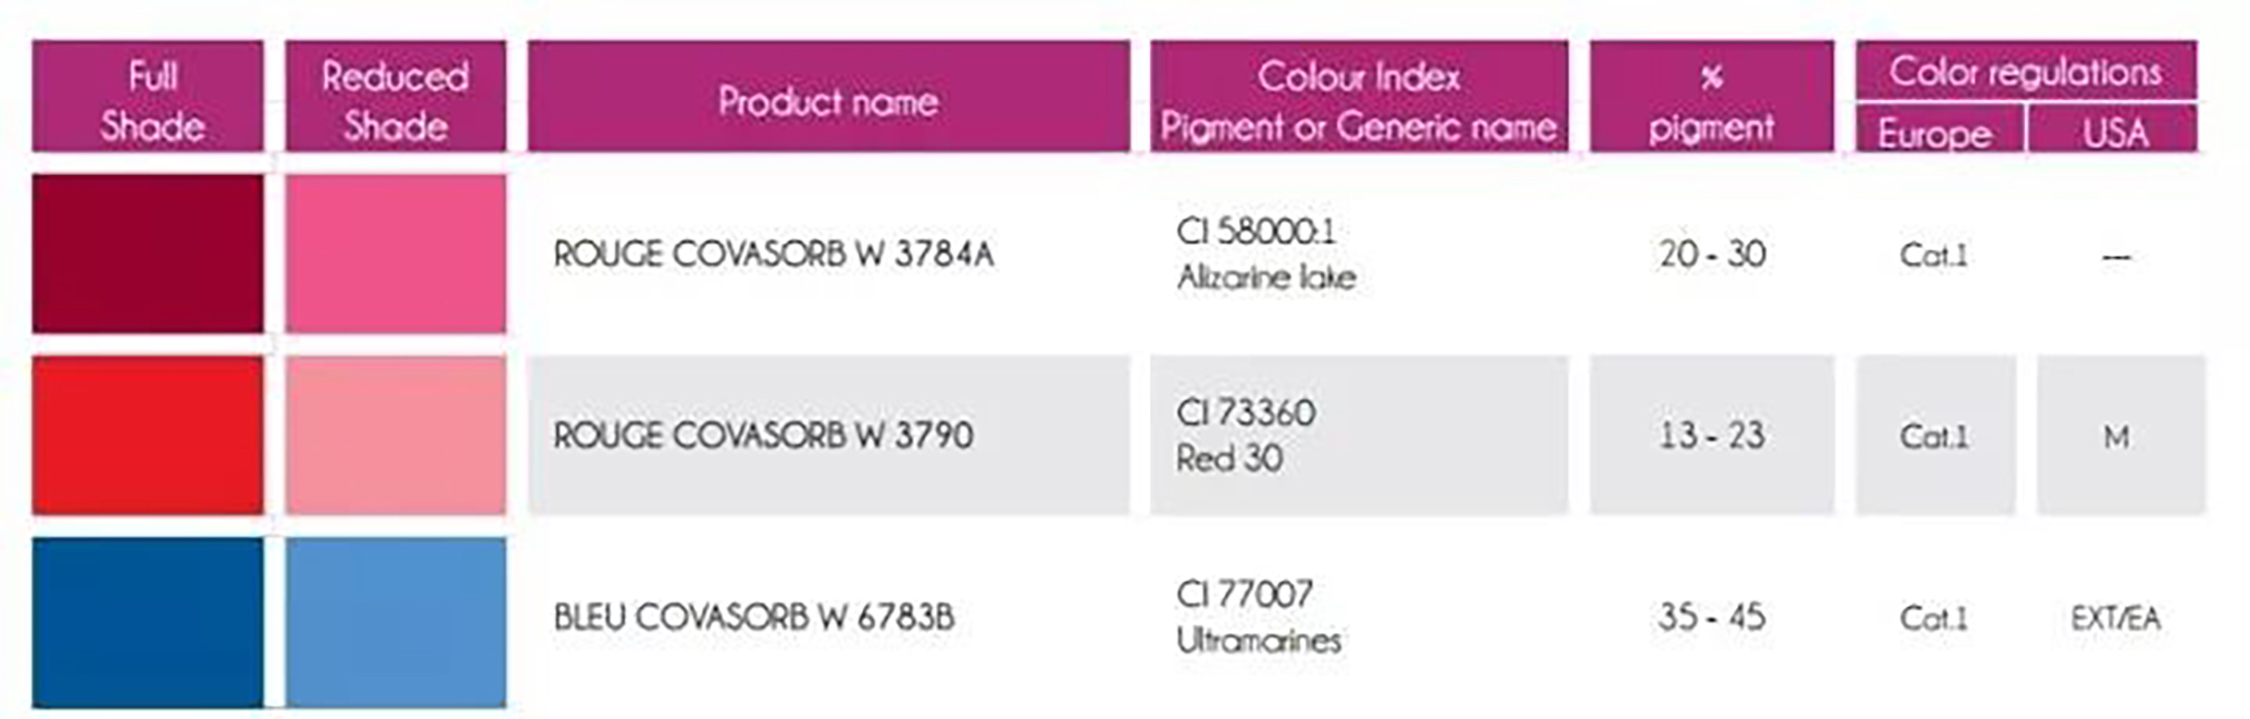
\includegraphics[width=0.9\linewidth]{IMG/201907/05.jpg}
    
    
\end{table}

\begin{multicols}{2}
\section*{在挤牙膏的时候,为什么不同颜色的彩条不会混合?}

刚才说到牙膏是一种宾汉流体.当你在挤牙膏的时候,彩条就会流动起来,变得更像液体而不是固体,这样它们才能从牙膏管子里流出.当牙膏流动的时候,它就必须要符合一个可怕的流体力学规律——\qiangdiao{雷诺数}(\textit{Reynolds number}\/).雷诺数的计算公式如下,开不开心,惊不惊吓?

\[
\begin{split}
\mathrm{Re}&=\mathrm{\frac{inertial\ forces}{viscous\ forces}}\\
&=\mathrm{\frac{mass \times acceleration}{dynamic\ viscousity\times \frac{velocity}{distance}\times area}}
\end{split}
\]

计算雷诺数的这个公式看看就好了,反正我们以后不考.它的意思是,一种流体的粘度(\textit{viscosity}\/)越大,它的雷诺数就越小;反之粘度越小,雷诺数就越大.雷诺数决定了液体是怎样流动的.

\begin{figure}[H]
    \centering
    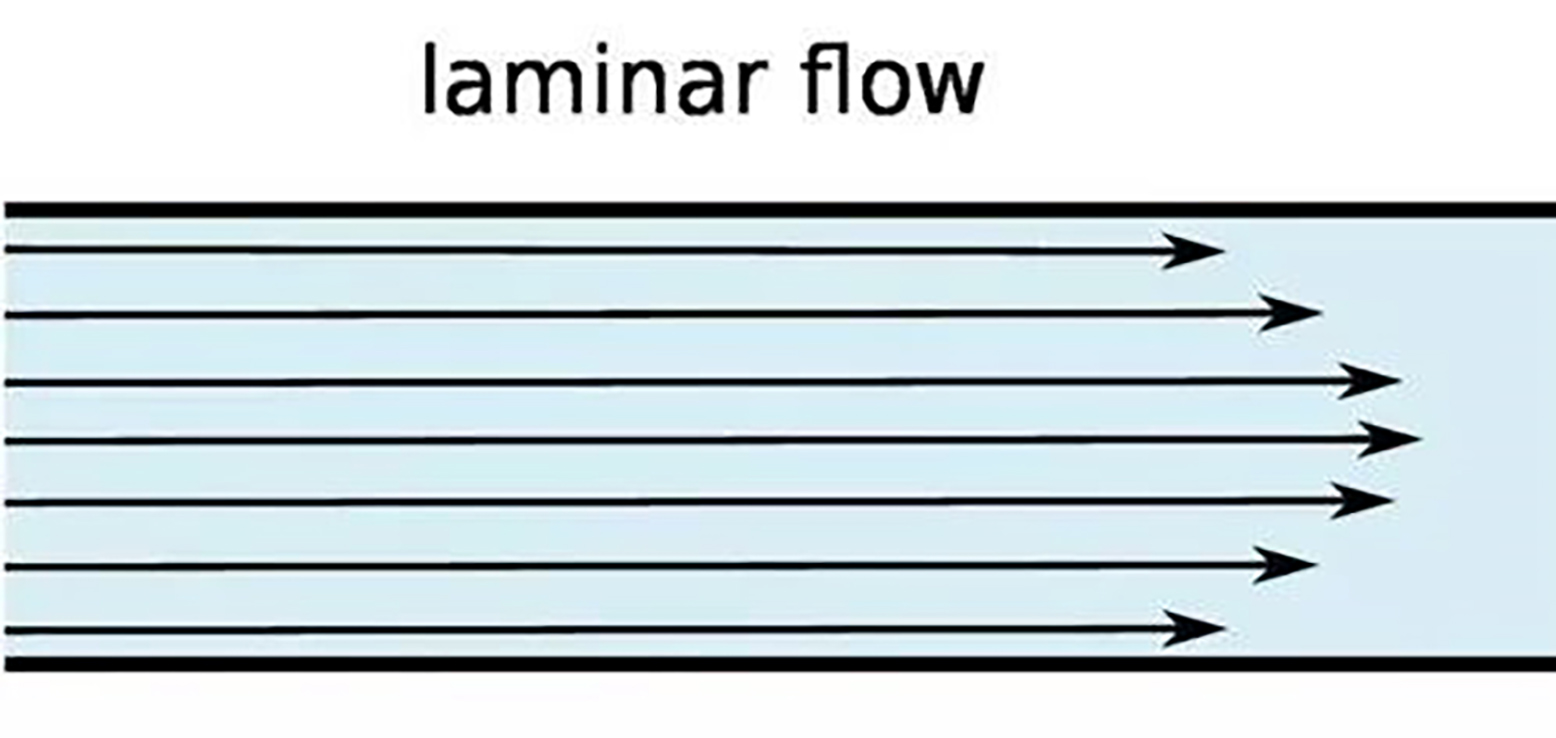
\includegraphics[width=0.5\linewidth]{IMG/201907/07.jpg}\\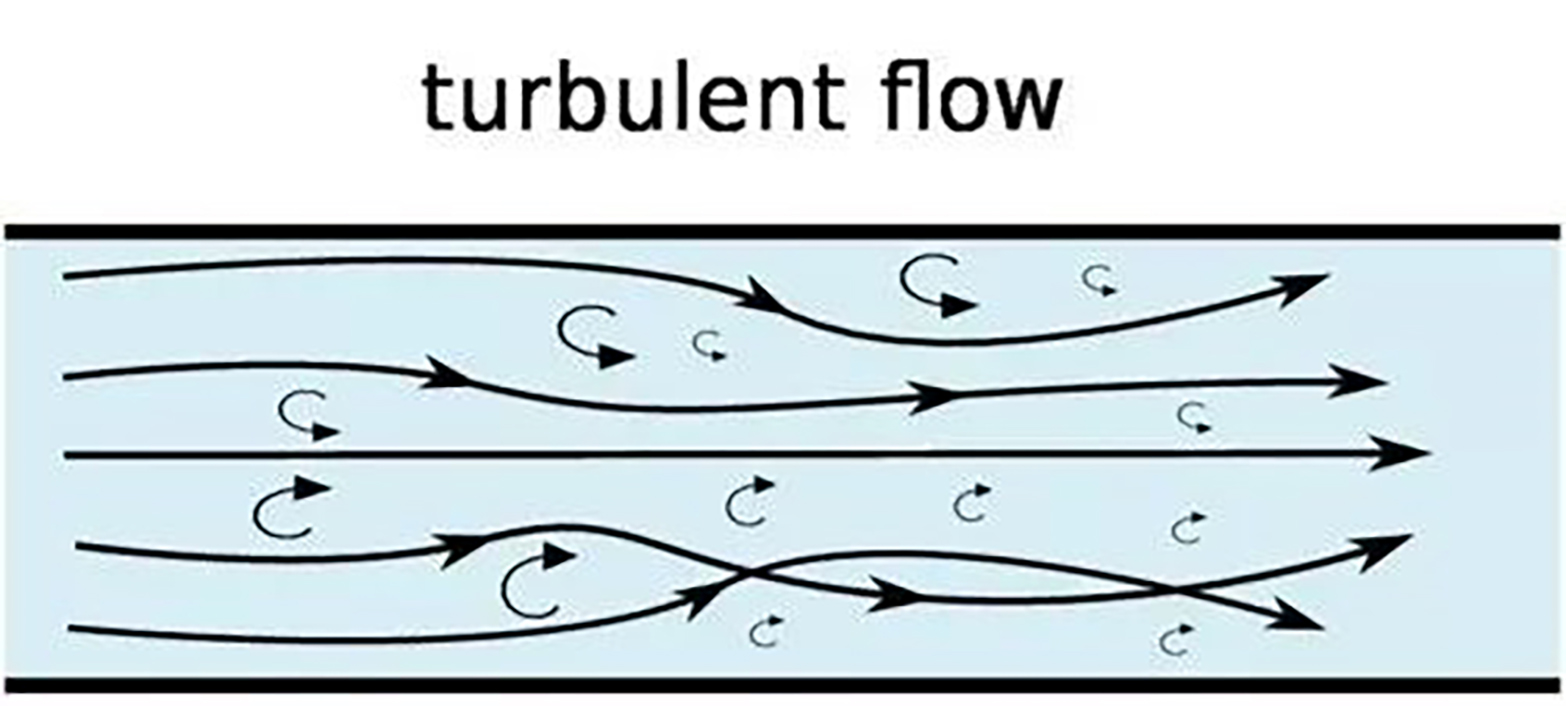
\includegraphics[width=0.5\linewidth]{IMG/201907/08.jpg}

    \caption{\textit{层流与湍流}}
    
\end{figure}




具体来说,如果雷诺数小于2100,那么液体将进行\qiangdiao{层流}(\textit{laminar flow}\/),层流的液体平行运动,不会搅和在一起.

如果雷诺数大于4000,那么液体将进行\qiangdiao{湍流}(\textit{turbulent flow}\/),看图就知道,湍流的液体互相混合.

\qiangdiao{对于牙膏来说,它的粘度非常大,因此它的流动只能是层流.}挤牙膏的时候,位于边缘的彩条和中间的白条一起平行流出,所以挤出来的牙膏彩条也不会混合在一起.当然了,牙膏和粘度较小的水混合后,雷诺数蹭蹭上涨,所以彩条的颜色就会混在一起,水乳交融了.最后,因为不同颜色的彩条有相同的流速(\textit{它们的流变学性质相同}),因此可以保证挤到最后也不会出现某种彩条被首先挤完的情况.

\section*{怎么保证挤到最后还有2种颜色的彩条?}

这是因为在这种牙膏里,红色彩条和白色彩条的粘度不同,红色彩条的粘度比较小,所以它更加顺滑,流得比较快.白色彩条的粘度更大,流得更慢.这两种不同粘度的彩条搭配以后,就能保证直到最后一滴,挤出来的牙膏都有两种颜色.不过,这种设计的销量并不好,后来逐渐被更加简单的设计,也就是我们现在使用的彩条牙膏替代了.
\end{multicols}

\noindent \qiangdiao{参考资料}

\noindent\url{[1]https://www.gsk.com/en-gb/behind-the-science/patients-consumers/science-of-a-different-stripe/}

\noindent\url{[2]https://bashny.net/t/en/91030}

\noindent\url{[3]https://www.sciencesetavenir.fr/fondamental/70-ans-de-sciences-et-avenir-le-secret-du-dentifrice-a-rayures\_116813}

\noindent\url{[4]https://www.youtube.com/watch?v=RVZ6mUffJgw}

\noindent\url{[5]https://www.britannica.com/science/laminar-flow}

\noindent\url{[6]https://www.archtoolbox.com/materials-systems/hvac/laminarflowvsturbulentflow.html}

\noindent\url{[7]http://www.russochemie.ru/upload/iblock/documents/Brochure\%20Cosmetic\%20Dispersions.pdf}

\noindent\url{[8]http://www.sensient-cosmetics.com/pageLibre000105e3.aspx}

\noindent\url{[9]http://ijppsjournal.com/Vol3Suppl3/2152.pdf}\vfill

\greybox{\vskip-25pt
\makeheading{生活中的科学}

\ \ \ \ 生活中,想必不少同学都会遇到一些“压不住牛顿的棺材板”的问题,那让我们一同浏览Question of the Month吧!

Q1.为什么放在一起的线不知不觉就缠在一起了?

Q2.用盆接水,离水龙头近,接满水更快,还是离得远的快?

Q3.为什么金属会有味道?

Q4.老人做豆腐时用嘴一吸水,水就一直流的原因是?

\centering{\qiangdiao{怎么样?有灵感了吗?快将你的思考分享给《星空》编辑部!}

\qiangdiao{答案将在下期揭晓哦}

\qiangdiao{主编}\ 蒋有为\ Wechat: \texttt{Jerry13616483961}\ \qiangdiao{副主编}\ 王鸿硕\ Wechat: \texttt{harrywanghs}}
}


\ADyixuehui
\newpage
\makeheading{科技快讯}
\begin{multicols}{2}
\section*{· 农业 ·}

\subsection*{严重威胁香蕉产业的TR4疑似蔓延至美洲}

{\centering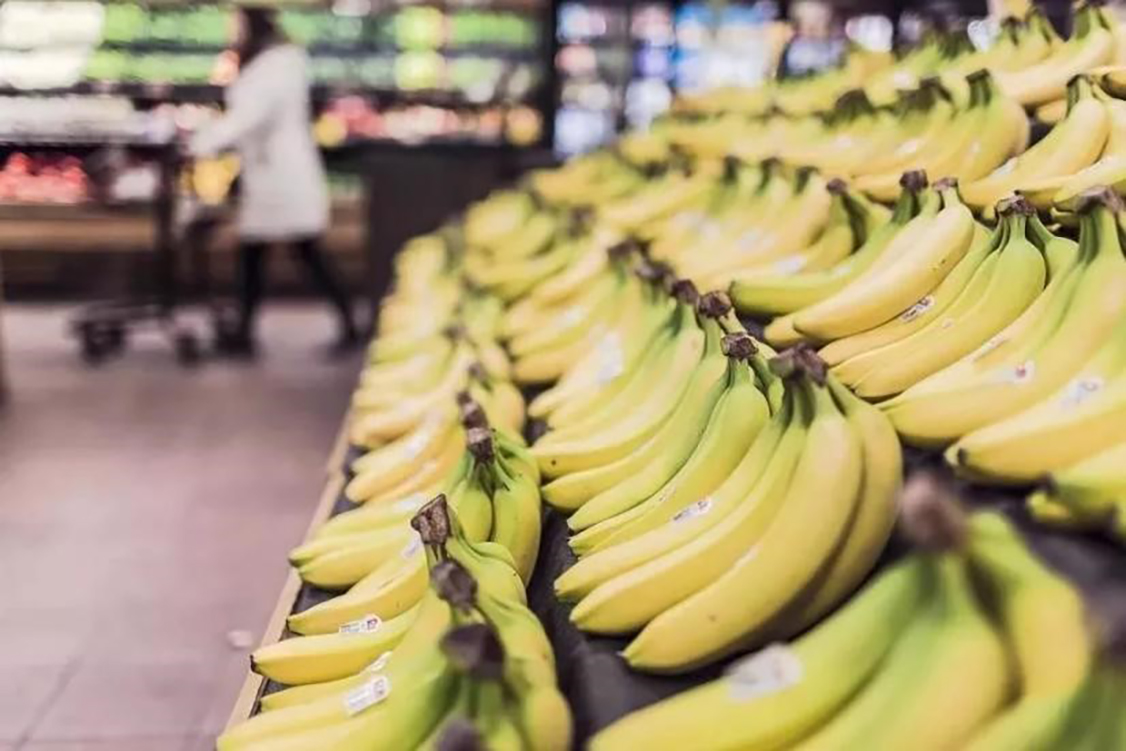
\includegraphics[width=0.8\linewidth]{IMG/201907/09.jpg}\vskip0cm}

上周,哥伦比亚农业研究所证实,该国北部四个种植园内的香蕉疑似感染了尖孢镰刀菌(TR4).这些种植园的香蕉样本被送往实验室进行基因组分析,最终分析结果将于8月初揭晓.这种真菌最早在东南亚地区被发现,并已传播至中东和非洲地区.由于香蕉对TR4几乎没有抗性,其大规模暴发将会给香蕉种植园带来毁灭性打击,并在全球范围内抬高香蕉价格.有学者指出,中美洲和南美洲的TR4很难控制,并且很多个体农户将承担不起控制措施.

\section*{· 遗传学 ·}

\subsection*{男女各个器官都存在差异表达基因}

男性与女性除了生殖方面的差异,也存在骨头、大脑等结构和器官的不同.更关键的是,男女容易患病的种类也不一样,比如女性更容易遭受自身免疫疾病,而男性患心血管疾病的风险要更高.发表在《科学》上的研究,按性别分类分析了四种哺乳动物的RNA序列,并与人类基因数据库进行了比较.它们发现,例如在控制身高的基因中,男女就有12\%的基因表达不一样.除此之外,在各个器官中,有数百个基因都展现出了性别差异表达.在未来,这些表达差异的基因对个性化治疗有极大参考价值.

\section*{· 纳米科学 ·}

\subsection*{具有永久磁性的液态磁铁}

{\centering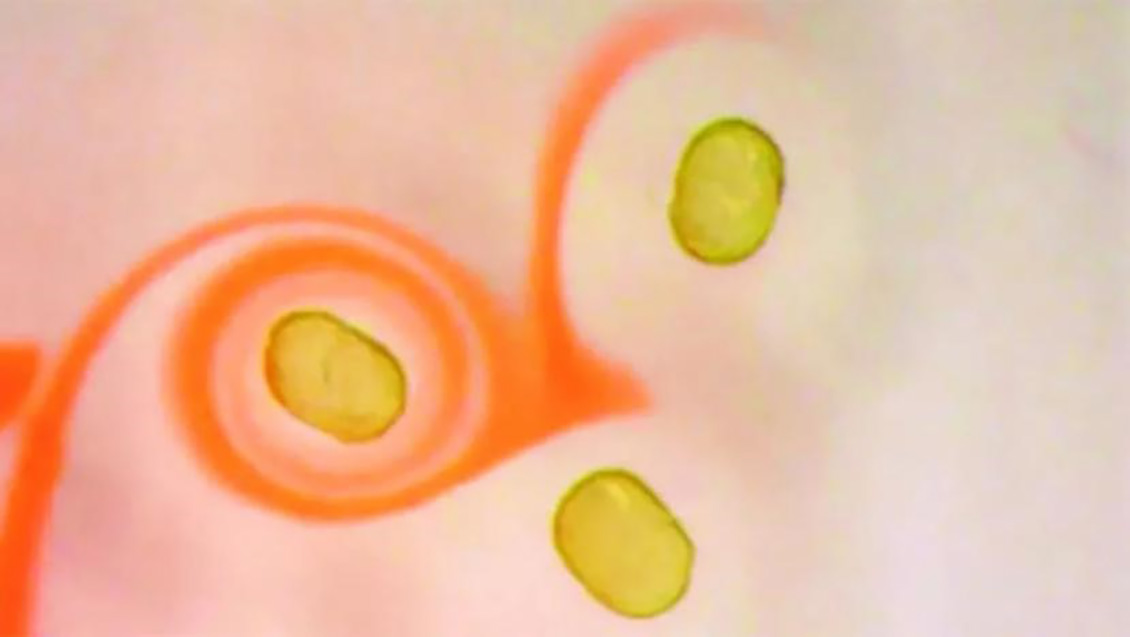
\includegraphics[width=0.8\linewidth]{IMG/201907/10.jpg}\vskip0cm}

在一项发表于《科学》杂志的最新研究中,中美研究团队采用全液相3D打印技术,制备出一种具有永久磁性的新型液滴.这种铁磁流体液滴直径约1毫米,由大量直径20纳米的氧化铁纳米颗粒组成.聚集在一起的纳米颗粒在磁性线圈的作用下,表现出磁性.当表面的纳米颗粒被磁化时,它们将磁性转移到中心的纳米颗粒,整个液滴就有了永久磁性.这项技术可应用于提供靶向癌症治疗的人工细胞、可变形的液体机器人等.

\section*{· 工程 ·}

\subsection*{可通过行走时膝盖弯曲发电的新装置}

在一项发表于《应用物理通讯》的研究中,中国香港中文大学的研究团队开发出一种可穿戴在腿上的发电设备,可以通过捕获人行走时膝盖弯曲产生的动能发电.该设备重量只有307克,穿戴这种设备的人以每小时4千米的速度行走时,设备输出功率为1.6微瓦特.研究人员认为,新的人体动能采集技术有望促进可穿戴设备发展,使可穿戴健康监测仪等实现“自供电”,使用者可以摆脱经常需要充电带来的不便.(\textbf{新华社})

\section*{· 航天 ·}

\subsection*{天宫二号完成任务,再入大气层烧毁}

{\centering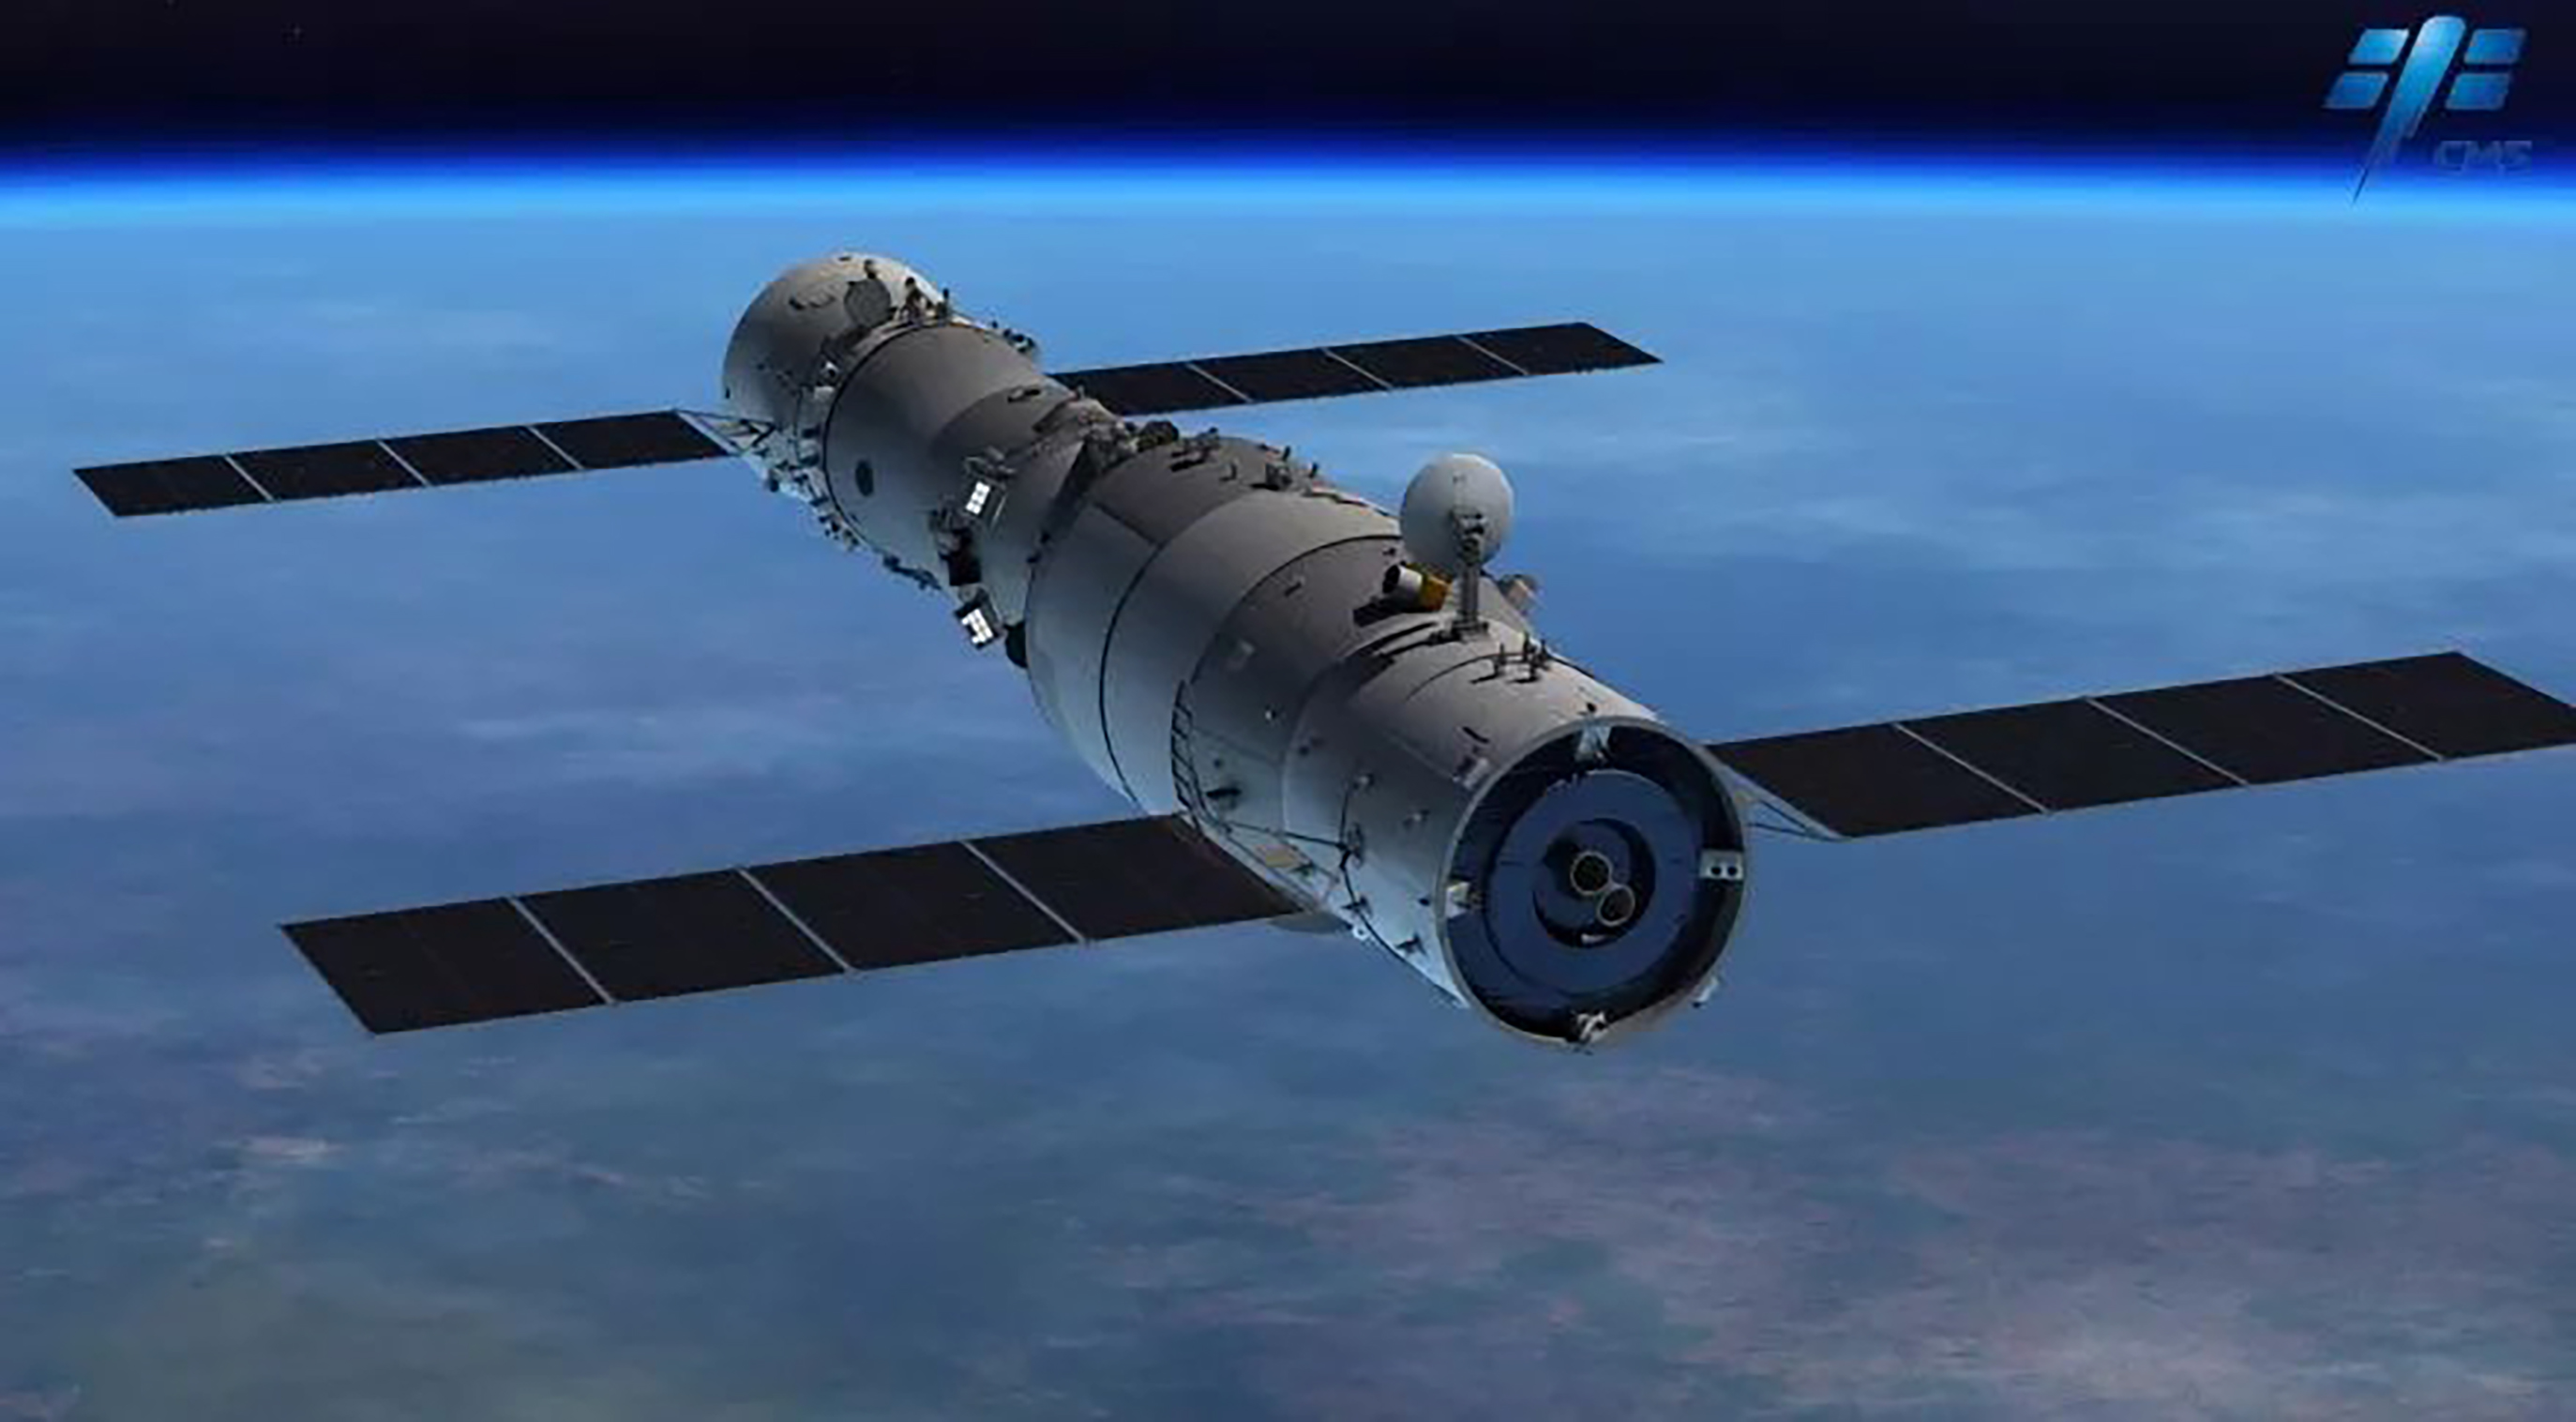
\includegraphics[width=0.8\linewidth]{IMG/201907/11.jpg}\vskip0cm}

2019年7月19日晚,天宫二号空间实验室成功受控离轨并再入大气层,少量残骸落入南太平洋预定安全海域.这标志着中国载人航天工程空间实验室阶段任务圆满完成.在超过1000天的飞行期间,天宫二号与神舟十一号、天舟一号进行了多次交会对接,并开展了一系列空间实验,验证了航天员中期驻留太空的能力、伴星技术、推进剂在轨补加技术等,为组建空间站奠定了基础.

\noindent \qiangdiao{参考链接}

\noindent\url{[1]https://mp.weixin.qq.com/s/g7PMKej1pcKz6NJTlV185g}
\end{multicols}\newpage
\makeheading{时空中的面积定律}
\begin{multicols}{2}
\qiangdiao{局域性}是所有物理的相互作用背后的一个基本原理.它说的是,每个物理系统只能与在它附近的其他系统进行相互作用,因此若两个相距遥远的物体之间要发生相互作用,则必须由某种中介来协调.例如,无线通信设备和移动电话能够在远距离发送和接收信息,而在其中起到中介作用的是电磁波.

同样地,在粒子物理学中,基本粒子(\textit{比如电子})也有着相似的行为.当两个相隔一定距离的基本粒子彼此施加作用力时,并不是在瞬间发生的,而是通过交换了一个粒子才实现的,这个粒子在局域中起到了传递力的作用.

物理的相互作用的局域性带来了一个重要的结果,那就是许多物理系统(\textit{从黑洞到量子多体系统})都满足一个特别的定律,即所谓的\qiangdiao{“面积定律”}.

为了解释这个属性的含义,假设有两个观察者$A$和$B$,他们对整个物理系统的组成部分进行测量.

\begin{figure}[H]
    \centering
    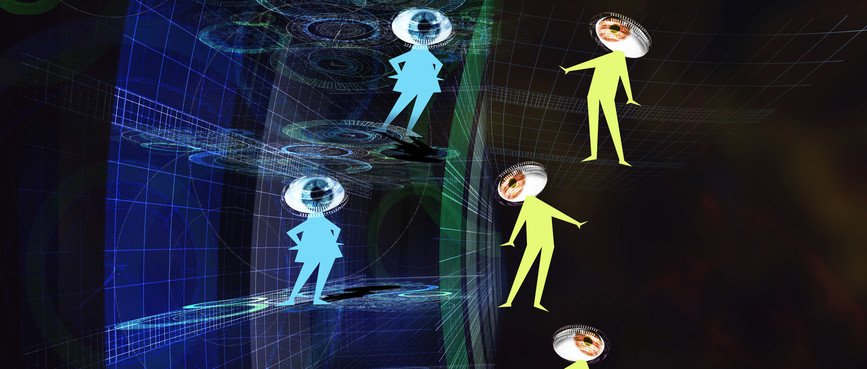
\includegraphics[width=\linewidth]{IMG/201907/csm_slider_quantenkorrelation_1920_2319fd8ab9.jpg}
    \caption{\textit{两个虚拟的观测者将时空和量子物理结合在了一起}}
    
\end{figure}



$A$只能测量空间中一个区域内的部分,一个边界将这个区域与其余部分隔开;而$B$可以对$A$的区域以外的部分进行测量.我们可以将“面积定律”粗略地解释为,它指的是$A$和$B$所测得结果的相互关联程度是由将$A$和$B$分割的边界面积决定的,而非区域的体积决定.这令人有些意外,因为许多其他与热力学或信息有关的物理量(\textit{如能量或熵等}),通常都是随体积变化的,而非面积.

虽然通常来说,面积定律会以空间区域的形式来表述,但将时间与空间统一为时空的相对论告诉我们,对物理的正确描述应该依据时空中的局域的相互作用.这就提出了一个问题,那就是面积定律性质是否可以被推广到时空中的区域.

现在,我们假设$A$可以访问某个系统的一部分,这个部分是被一个盒子所限制的空间.$A$可以在有限的时间内在这个空间中进行多次测量.这样一来,她所有的测量都是在一个四维的时空盒中进行的.$B$可以在$A$的盒子之外的时空中的任意一点访问系统.

在一篇发表于《NPJ | 量子信息》的新论文中,物理学家研究了这个四维时空的边界地区是否能告诉我们一些关于$A$和$B$的测量结果之间的相关性程度的信息.

\begin{figure}[H]
    \centering
    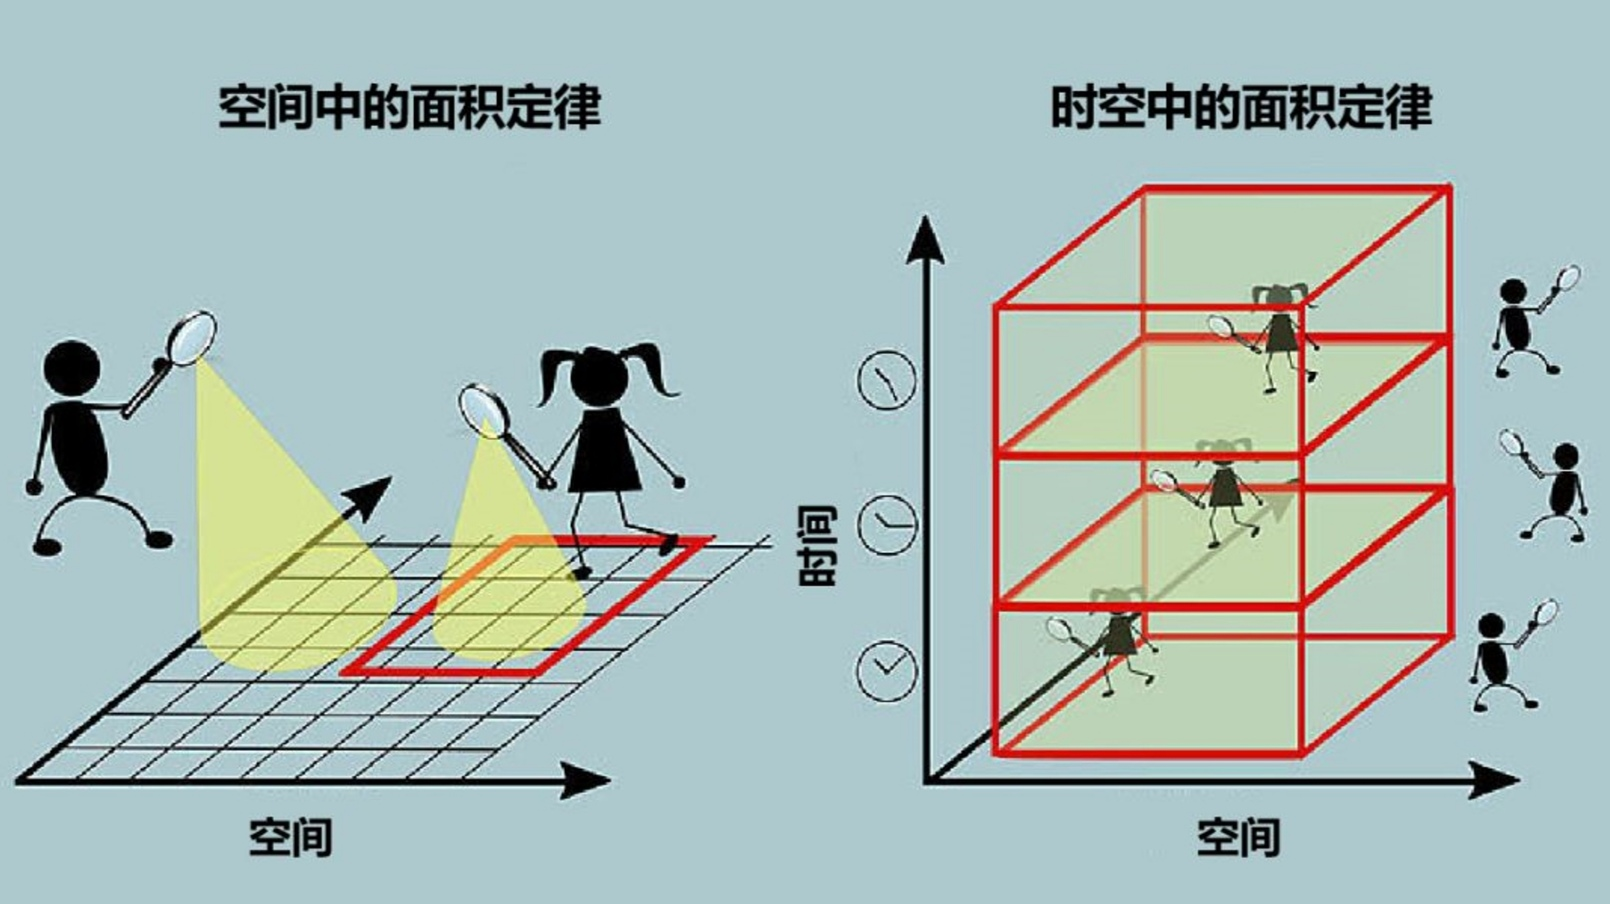
\includegraphics[width=\linewidth]{IMG/201907/Screenshot_20190725_152404.jpg}
    \caption{\textit{新的研究将这些结果扩展到了时空中.在时空中,$A$需要在一段时间内执行她的测量.结果是:即使在时空中,面积定律仍然适用,而且其相关性的强度取决于$A$进行测量的区域面积.}}
    
\end{figure}

在新研究中,物理学家指出,如果一个物理系统是由局域相互作用的粒子组成,那么在时空区域的面积定律依然是成立的.卡斯拉夫·布鲁克内尔(Ĉaslav Brukner)是论文的作者之一,他说:“这项研究为量子关联和时空几何之间提供了一种联系.这将有助于发展能将量子力学和引力统一起来的理论.”
\end{multicols}\vfill

\noindent\qiangdiao{原文链接}

\noindent\url{[1]https://www.oeaw.ac.at/en/detail/news/a-connection-between-quantum-correlations-and-spacetime-geometry/}\vfill

\ADhairui





